% Created 2023-12-08 Fri 18:07
% Intended LaTeX compiler: xelatex
\documentclass{beamer}
\usepackage{graphicx}
\usepackage{longtable}
\usepackage{wrapfig}
\usepackage{rotating}
\usepackage[normalem]{ulem}
\usepackage{amsmath}
\usepackage{amssymb}
\usepackage{capt-of}
\usepackage{hyperref}
\usepackage{ctex}
\usetheme{default}
\usetheme{default}
\author{方真}
\date{2023-12-05}
\title{开源软件与软件工程}
\AtBeginSection[]{\begin{frame}<beamer>\frametitle{目录}\tableofcontents[currentsection]\end{frame}}
\hypersetup{
 pdfauthor={方真},
 pdftitle={开源软件与软件工程},
 pdfkeywords={},
 pdfsubject={},
 pdfcreator={Emacs 29.1 (Org mode 9.6.6)}, 
 pdflang={English}}
\begin{document}

\maketitle

\section{开源基础概念}
\label{sec:org2f5f59c}
\begin{frame}[label={sec:org4c16e6a}]{什么是开源软件}
开源软件是指源代码对公众开放,允许自由使用、复制、修改和分发的软件
\begin{itemize}
\item 开放源代码:软件的源代码对任何人都是可用的,可以被查看和修改
\item 透明性与可验证性
\item 开放的设计与开发过程
\item 遵循开源协议
\end{itemize}
\end{frame}
\begin{frame}[label={sec:orga97a4b0}]{OSI对开源软件定义}
\begin{itemize}
\item 自由分发
\item 源代码开放
\item 允许修改和派生
\item 作者源代码的完整性
\item 不歧视任何个人或团体
\item 不歧视任何特定用途
\item 许可协议的分发:无需额外许可即可使用
\item 许可协议不局限于某个产品
\item 许可协议不得限制其他软件
\item 许可协议必须保持技术中立
\end{itemize}
\end{frame}
\begin{frame}[label={sec:org57c58ce}]{FSF对自由软件的定义}
\begin{itemize}
\item 基于任何目的使用该软件的自由
\item 研究软件如何工作,修改软件的自由
\item 重分发该软件的自由
\item 重分发派生版本的自由
\end{itemize}
\end{frame}
\begin{frame}[label={sec:orgcea1471}]{开源软件简史}
\begin{itemize}
\item 早期软件著作权从无到有
\item Unix与C语言的诞生:60年代末到70年代初
\begin{itemize}
\item 源码可近乎免费获得,可用于非商业用途
\end{itemize}
\item 70到80年代:越来越多的公司将软件作为财产,源码受保护,无法免费获取
\begin{itemize}
\item 1976 比尔盖茨 《致爱好者的公开信》
\end{itemize}
\item 80到90年代,随着AT\&T对SystemV 商业版收费和限制,BSD Unix逐步发展起来
\begin{itemize}
\item 至今OpenBSD/NetBSD/FreeBSD依然在开发
\end{itemize}
\item 1983年,Richard Stallman发起了GNU计划
\item 1991年,Linus发布第一版Linux内核。GNU/Linux成为了一个完全自由的开源操作系统
\item 1998年,Eric Raymond 和 Bruce Perens成立了开源促进组织(Open Source Initiative)。
\item 2004年,中国开源软件推进联盟成立
\item 2020年,开放原子开源基金会成立,是中国内地首个开源领域的基金会
\end{itemize}
\end{frame}

\begin{frame}[label={sec:org62b9030}]{开源许可证}
开源许可证可以粗略地分为两大类:
\begin{itemize}
\item 著佐权许可证 ("Copyleft license")
\begin{itemize}
\item 在软件被修改并再发行时,仍然强制要求公开源代码
\end{itemize}
\item 宽松自由软件许可协议 ("Permissive free software licence")
\begin{itemize}
\item 衍生软件可以变为专有软件
\end{itemize}
\begin{center}
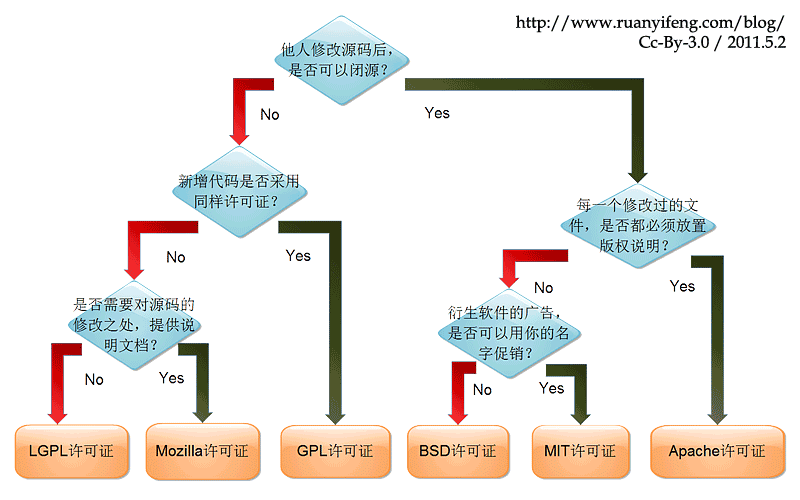
\includegraphics[width=.9\linewidth]{../assets/static/opensource/license.png}
\end{center}
\end{itemize}
\end{frame}

\begin{frame}[label={sec:orgc98b2f2}]{开源软件的例子}
\begin{itemize}
\item 操作系统内核:Linux、BSD、AOSP
\item 浏览器:Firefox、Chromium
\item 数据库:Mariadb、PostgreSQL
\item 云计算:Openstack、Kubernetes
\item 虚拟化:Qemu、Bochs
\item 编程语言:Java、Python、Go、Rust
\item 编译器:GCC、LLVM
\item Web 服务器:Httpd、Nginx
\item 开发工具:Git、Eclipse、Emacs、Vi
\item Web \& 桌面:Angular、Vue.js、Flutter
\item AI框架:TensorFlow、Pytorch
\item 多媒体:FFmpeg、VLC
\item 科学计算:NumPy
\end{itemize}
\end{frame}

\section{开源项目中的软件工程}
\label{sec:org4e077ee}
\begin{frame}[label={sec:orgfc3bc9a}]{开源软件工程实践的特点}
总的来说,开源项目中的软件工程实践强调了社区参与、透明度、协作和持续交付,这些特点使得开源项目具有更强的创新能力和灵活性。
\begin{itemize}
\item 分散的开发者群体
\item 透明度和公开性
\item 社区参与和治理
\item 持续集成和持续交付(CI/CD)
\item 开放式问题跟踪和协作
\item 文档的重要性
\item 代码评审和协作
\end{itemize}
\end{frame}
\begin{frame}[label={sec:orgfc9f4fd}]{案例:Openstack项目}
OpenStack是一个开源的云计算平台,旨在提供基础设施即服务(IaaS)和平台即服务(PaaS)解决方案。
由Open Infrastructure Foundation 负责运营。
许可协议采用Apache 2.0。
\end{frame}

\begin{frame}[label={sec:orgd7a7f74}]{治理与组织结构}
\begin{itemize}
\item 董事会
对OpenStack基金会以及基金会所保护的资产 (如OpenStack商标) 进行监督。
由赞助商指定以及选举产生。
\item 技术委员会(TC)
OpenStack项目的最高技术决策机构。TC成员由选举产生,负责项目技术方向、标准、项目治理规则等决策。
\item 用户委员会
用户委员会代表用户利益,与其他方进行合作,确保Openstack项目方向符合用户需求。
\item 项目团队
\begin{itemize}
\item OpenStack项目被组织成一系列的项目组,每个项目组负责一个或多个相关的项目。
\item 每个项目组都有一个项目组长 (Project Team Lead,PTL) 负责组织和协调项目组的活动。
\item 每个项目组都有多个Core Reviewer
\end{itemize}
\end{itemize}
\end{frame}

\begin{frame}[label={sec:org45f7cc4}]{项目管理}
\begin{itemize}
\item Openstack项目是一直发展的,从最初的Nova到现在几十个项目。
\item 新项目的准入是由TC来评估和决定;同时项目开发者可以获得TC的投票权。
\item 必须满足Openstack要求(4 Opens):
\begin{itemize}
\item 开放源码
\item 开放社区
\item 开放开发
\item 开放设计
\end{itemize}
\item Openstack的项目管理机制几经变化,目前流程有所简化。
\end{itemize}
\end{frame}

\begin{frame}[label={sec:orgf9e0d31}]{Feature管理}
\begin{itemize}
\item Blueprint在Openstack项目中用来追踪重大特性的实现。
\begin{itemize}
\item 包含了详细规划和设计文档。
\item 由社区成员创建,并经过讨论、审查和批准。
\end{itemize}
\item Blueprint的生命周期:
\begin{itemize}
\item 提出与创建,上传设计文档到代码库;
\item Blueprint被批准,其中会经过讨论与反馈,修改与评审;
\item 由提出者或其他人实现,并保持进度更新;
\item 需求实现,状态变成完成
\end{itemize}
\end{itemize}
\end{frame}

\begin{frame}[label={sec:orgf66b3fc}]{Bug追踪系统}
Openstack项目使用launchpad来进行bug与任务追踪。
\begin{itemize}
\item 通常来说,Bug要有以下几个信息:
\begin{itemize}
\item Bug基本信息:现象、触发条件等
\item 状态
\item 优先级
\item 报告人和负责人
\item 目标版本,受影响版本
\item 其他标签
\end{itemize}

\item Bug的主要生命周期
\begin{itemize}
\item 报告
\item 确认优先级
\item 修复方案的实现
\item 完成
\end{itemize}
\end{itemize}
\end{frame}

\begin{frame}[label={sec:org296ec85}]{沟通与文档}
开源项目的协作模式决定了它不同于商业软件的沟通方式。
沟通主要发生在:
\begin{itemize}
\item 开发者和社区内部
\item 外部用户与开发者
\end{itemize}
沟通方式:
\begin{itemize}
\item 各种需求管理,任务追踪系统
\item 即时通信
\item 邮件列表
\item 文档
\begin{itemize}
\item 文档在开源项目中处于核心地位
\item 高质量的文档对于开源项目有巨大的助益
\end{itemize}
\end{itemize}
\end{frame}

\begin{frame}[label={sec:org529bf66}]{代码托管与评审}
\begin{itemize}
\item Openstack项目采用Gerrit来管理代码。
\begin{itemize}
\item Gerrit是一个基于Git的代码评审和管理系统
\item 一切皆可代码化
\end{itemize}
\item 代码都需要经过评审才能进入代码库
\begin{itemize}
\item 每个patch提交之后都会自动执行自动化测试
\item 贡献者可以邀请其他人参与评审
\item 项目的 Core Reviewer 需要同意
\end{itemize}
\item 分支模型
\end{itemize}
\end{frame}

\begin{frame}[label={sec:org1e63c5a}]{生态}
\begin{itemize}
\item 赞助商:Openstack 赞助商分为白金赞助商,黄金赞助商,白银赞助商
\item 发行版:Redhat、Canonical、华为等
\item OpenInfra 峰会
\item COA认证与培训
\item 用户:2022年数据,全球300个公有云数据中心,4000万 CPU Core 的部署规模
\end{itemize}
\end{frame}

\section{开源软件的软件工程挑战}
\label{sec:orgd101a9b}
\begin{frame}[label={sec:org5e725f7}]{}
\begin{center}
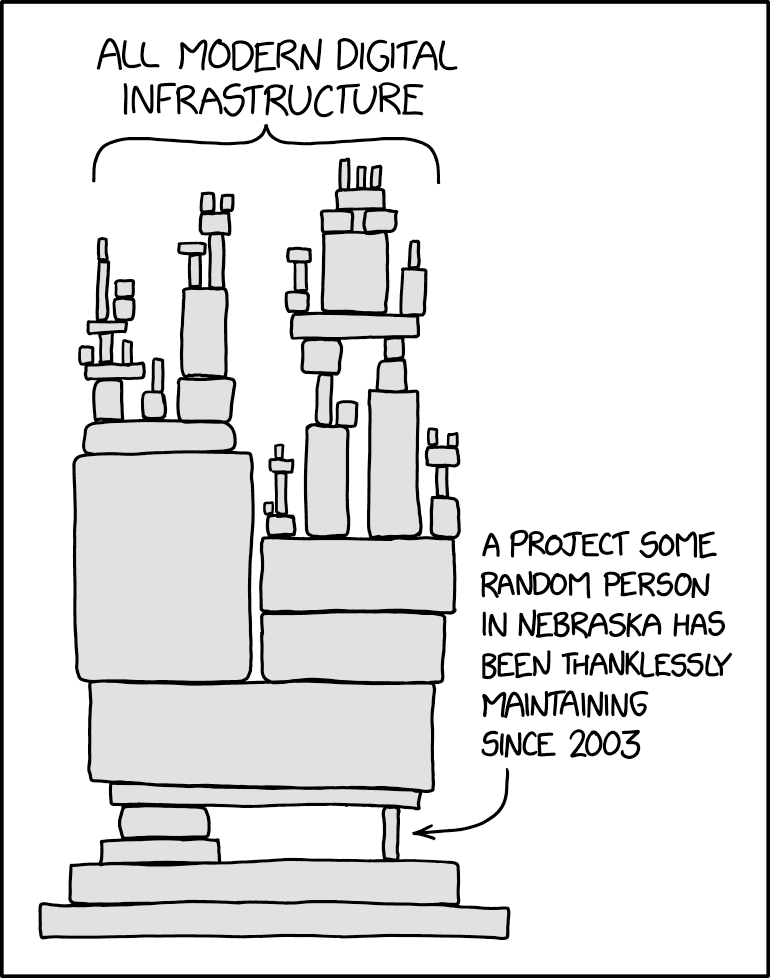
\includegraphics[height=\textheight]{../assets/static/opensource/fragile.png}
\end{center}
\end{frame}

\begin{frame}[label={sec:org6714fa2}]{实例:OpenSSL heartbleed漏洞}
Heartbleed是OpenSSL的一个严重漏洞,它允许攻击者在正常情况下窃取本应受SSL协议加密保护的信息。
\begin{itemize}
\item Heartbleed是OpenSSL在心跳机制的代码实现中产生的漏洞,并非SSL协议中的设计缺陷。
\item OpenSSL可能是使用最广泛的SSL/TLS实现:
\begin{itemize}
\item nginx、apache httpd都使用OpenSSL,两者合计占有一半以上的Web server市场
\item 众多Linux发行版和BSD发行版都包含OpenSSL
\end{itemize}
\item 漏洞2012年引入,2014年4月公开。期间可能有未被披漏的利用。
\end{itemize}

类似问题
\begin{itemize}
\item log4j漏洞:CVE-2021-44228
\item core-js维护问题:\url{https://github.com/zloirock/core-js/blob/master/docs/2023-02-14-so-whats-next.md}
\end{itemize}
\end{frame}

\begin{frame}[label={sec:org3225c3e}]{挑战:项目本身}
\begin{itemize}
\item 项目开发过程
\begin{itemize}
\item 代码风格与质量
\item 核心开发者的开放性
\end{itemize}
\item 资源有限
\item 项目运营
\begin{itemize}
\item 成功的项目需要重视代码之外的建设
\end{itemize}
\item 问题修复和通知的挑战
\end{itemize}
\end{frame}

\begin{frame}[label={sec:org40d9e20}]{挑战:项目之外}
\begin{itemize}
\item 广泛影响
\item 关注依赖链的复杂性
\item 及时关注并修复安全漏洞
\item 选取开源项目时的评估
\item 赞助开源项目,促进良性发展
\end{itemize}
\end{frame}

\begin{frame}[label={sec:orge9ddf51}]{没有银弹}
开源软件有虽然诸多优势,但并不能解决软件开发的所有问题。
\begin{itemize}
\item 项目可持续性
\item 安全风险
\item 许可问题
\begin{itemize}
\item Redis、Mongo许可变更
\end{itemize}
\item 版本兼容性
\begin{itemize}
\item 开源项目对兼容性的哲学与商业目标不一定一致
\end{itemize}
\item 社区支持有限
\begin{itemize}
\item 当缺乏足够的技能解决开源项目的问题时,无法像商业软件一样寻求支持
\end{itemize}
\item 过时的版本
\begin{itemize}
\item 91%的商业软件包含过时或废弃的开源组件
\item 升级难度
\end{itemize}
\item 社区分裂
\begin{itemize}
\item MariDB vs. MySQL
\item 派生版本与主线开源版本分裂
\end{itemize}
\end{itemize}
\end{frame}

\begin{frame}[label={sec:org343f85b}]{业界方案}
开源生态产品化:
将开源软件或技术整合到一个完整的产品或解决方案中,并通过商业化的方式提供给最终用户或企业。
\begin{itemize}
\item 商业支持和服务
\item 可扩展性和定制性
\item 安全性和合规性
\item 用户友好的界面
\end{itemize}

软件工程在开源生态产品化中发挥着关键作用
\begin{itemize}
\item 通过软件工程的系统性思维来解决产品化过程中的问题
\item 着眼于整个产品和方案,而不只是具体的代码实现
\item 可维护性是软件生命周期的一个重要而关键的阶段
\end{itemize}
\end{frame}

\section{参与开源项目}
\label{sec:org564f51f}
\begin{frame}[label={sec:org00e1e2d}]{参与理由}
参与开源项目是学习和实践软件工程的绝佳选择
\begin{itemize}
\item 获得实际项目经验
\begin{itemize}
\item 了解真实世界的软件开发挑战和流程
\item 比教科书学习更加深入的体验
\item 可以实践软件工程的方法学
\end{itemize}
\item 锻炼协同合作的能力
\begin{itemize}
\item 能够与来自不同背景和地区的开发者合作
\end{itemize}
\item 提升技术能力
\begin{itemize}
\item 养成良好的设计和编程习惯
\item 学习新技术
\end{itemize}
\end{itemize}
\end{frame}

\begin{frame}[label={sec:orgd6f25ef}]{几点建议}
\begin{itemize}
\item 保持平常心
\item 了解并融入社区文化和技术风格
\item 选择感兴趣的项目
\item 动手而不是观望
\item 多样化贡献
\begin{itemize}
\item 编码、文档、测试、基础设施、提交反馈
\end{itemize}
\item 参与面向学生的开源活动
\begin{itemize}
\item 如开源之夏:中科院软件所发起并支持
\end{itemize}
\end{itemize}
\end{frame}

\begin{frame}[label={sec:org4a4c1ab}]{真实世界的软件开发流程}
\begin{center}
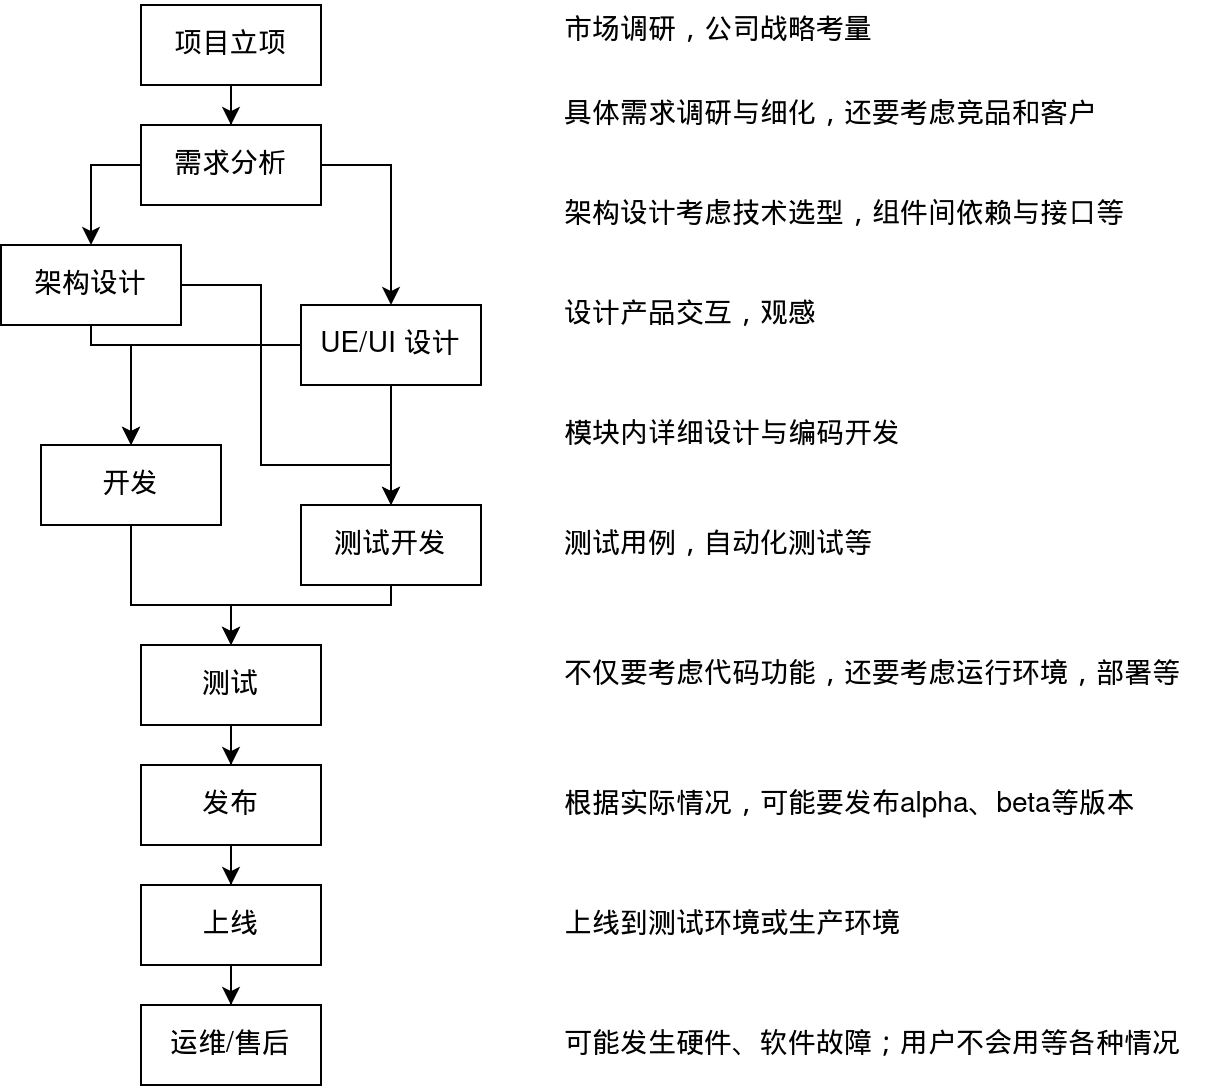
\includegraphics[height=0.9\textheight]{../assets/static/opensource/workflow.png}
\end{center}
\end{frame}

\begin{frame}[label={sec:org7b57a75}]{}
\begin{center}
\Huge Thank You!
\end{center}
\end{frame}

\begin{frame}[label={sec:org26c43b0}]{}
\begin{center}
\Huge Q\&A
\end{center}
\end{frame}
\end{document}